% !TeX root = Protokoll.tex


\section{Magnetisches Moment eines Elektrons}
Ein Elektron im Atom besitzt zu einem den Bahndrehimpuls $\vec{l}$ und zum anderen wie ein Eigendrehimpuls fungierenden Spin $\vec{s}$.
Die Beträge dieser vektoriellen Größen werden bestimmt durch
\begin{align}
	|\vec{l}|=&\sqrt{l(l+1)}\hbar\\
	\nonumber &\text{und}\\
	|\vec{s}|=&\sqrt{s(s+1)}\hbar.
\end{align}
Dabei sind $l$ und $s$ die Quantenzahlen, sowie $\hbar$ das Plancksche Wirkungsquantum.
Aufgrund der Ladung der Elektronen, entsteht da durch magnetische Momente $\vec{\mu_l}$ und $\vec{\mu_s}$ .
Mithilfe des Bohrschen Magnetons 
\begin{align}
	\mu_B:=-\frac{1}{2}e_0 \frac{\hbar}{m_0},
\end{align}
lassen sich diese Momente berechnen durch
\begin{align}
	\vec{\mu}_l=&-\mu_B\sqrt{l(l+1)}\vec{e}_l\\
	\nonumber &\text{und}\\
	\vec{\mu}_s=&-g_s\,\mu_B\sqrt{s(s+1)}\vec{e}_s.
\end{align}
Hier sind ist $e_0$ die Elementarladung, $m_0$ die Elektronmasse.
Weiter wird für $\vec{\mu}_s$ der Landé-Faktor eingeführt, der die Stärke der der Kopplung des Spins ans magnetische Moment beschreibt.


\subsection{Vorbereitungaufgaben}
\newpage
\FloatBarrier
\begin{figure}[!h]
\centering
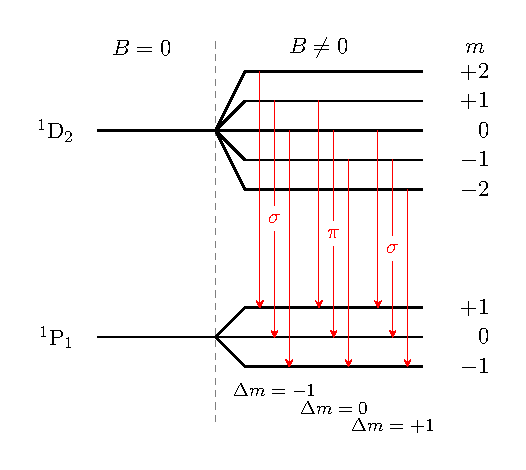
\includegraphics[scale=1.15]{../Grafiken/termschema_rot.pdf}
\caption{Hier ist das Termschema der roten Spektrallinie einer Cd-Lampe dargestellt\label{fig:termschema_rot}}
\end{figure}
\FloatBarrier
\FloatBarrier
\begin{figure}[!h]
\centering
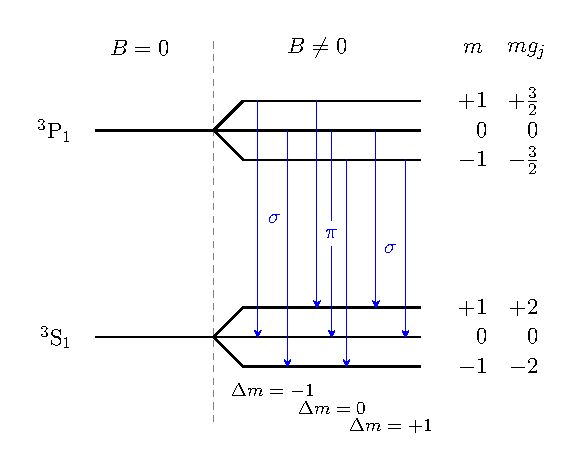
\includegraphics[scale=1.25]{../Grafiken/termschema_blau.pdf}
\caption{\label{fig:termschema_blau}}
\end{figure}
\FloatBarrier